\documentclass{sigchi-ext}
% Please be sure that you have the dependencies (i.e., additional
% LaTeX packages) to compile this example.
\usepackage[T1]{fontenc}
\usepackage{textcomp}
\usepackage[scaled=.92]{helvet} % for proper fonts
\usepackage{graphicx} % for EPS use the graphics package instead
\usepackage{balance}  % for useful for balancing the last columns
\usepackage{booktabs} % for pretty table rules
\usepackage{ccicons}  % for Creative Commons citation icons
\usepackage{ragged2e} % for tighter hyphenation
\usepackage{cite}

% Para adicionar a língua (PT)
\usepackage[portuges]{babel}
% suporte para utf8
\usepackage[utf8]{inputenc}

% Some optional stuff you might like/need.
% \usepackage{marginnote} 
% \usepackage[shortlabels]{enumitem}
% \usepackage{paralist}
% \usepackage[utf8]{inputenc} % for a UTF8 editor only

%% EXAMPLE BEGIN -- HOW TO OVERRIDE THE DEFAULT COPYRIGHT STRIP --
% \copyrightinfo{Permission to make digital or hard copies of all or
% part of this work for personal or classroom use is granted without
% fee provided that copies are not made or distributed for profit or
% commercial advantage and that copies bear this notice and the full
% citation on the first page. Copyrights for components of this work
% owned by others than ACM must be honored. Abstracting with credit is
% permitted. To copy otherwise, or republish, to post on servers or to
% redistribute to lists, requires prior specific permission and/or a
% fee. Request permissions from permissions@acm.org.\\
% {\emph{CHI'14}}, April 26--May 1, 2014, Toronto, Canada. \\
% Copyright \copyright~2014 ACM ISBN/14/04...\$15.00. \\
% DOI string from ACM form confirmation}
%% EXAMPLE END

% Paper metadata (use plain text, for PDF inclusion and later
% re-using, if desired).  Use \emtpyauthor when submitting for review
% so you remain anonymous.
\def\plaintitle{Eco Footprint - Understanding my impact} \def\plainauthor{João Nogueira, João Pina, Manuel Sousa,
  Miguel Regouga}
\def\emptyauthor{}
\def\plainkeywords{Ecology, footprint, internet of things}
\def\plaingeneralterms{Documentation, Standardization}

\title{Eco Footprint - Understanding my impact}

\numberofauthors{6}
% Notice how author names are alternately typesetted to appear ordered
% in 2-column format; i.e., the first 4 autors on the first column and
% the other 4 auhors on the second column. Actually, it's up to you to
% strictly adhere to this author notation.
\author{%
  \alignauthor{%
    \textbf{João Nogueira}\\
    \affaddr{Student number: 83488} \\
    \affaddr{Instituto Superior Técnico} \\
    \email{jrnogueira@edu.ulisboa.pt} }\alignauthor{%
    \textbf{João Pina}\\
    \affaddr{Student number: 85080}\\
    \affaddr{Instituto Superior Técnico}\\
    \email{joaomfpina@tecnico.ulisboa.pt} } \vfil \alignauthor{%
    \textbf{Manuel Sousa}\\
    \affaddr{Student number: 84740}\\
    \affaddr{Instituto Superior Técnico}\\
    \\
    \email{manuelvsousa@tecnico.pt} }\alignauthor{%
    \textbf{Miguel Regouga}\\
    \affaddr{Student number: 83530}\\
    \affaddr{Instituto Superior Técnico}\\
    \email{miguelregouga@tecnico.ulisboa.pt} } \vfil}

% Make sure hyperref comes last of your loaded packages, to give it a
% fighting chance of not being over-written, since its job is to
% redefine many LaTeX commands.
\definecolor{linkColor}{RGB}{6,125,233}
\hypersetup{%
  pdftitle={\plaintitle},
%  pdfauthor={\plainauthor},
  pdfauthor={\emptyauthor},
  pdfkeywords={\plainkeywords},
  bookmarksnumbered,
  pdfstartview={FitH},
  colorlinks,
  citecolor=black,
  filecolor=black,
  linkcolor=black,
  urlcolor=linkColor,
  breaklinks=true,
}

% \reversemarginpar%

\begin{document}

%% For the camera ready, use the commands provided by the ACM in the Permission Release Form.
\CopyrightYear{2019}
\setcopyright{rightsretained}
\conferenceinfo{CHI'20,}{April  25--30, 2020, Honolulu, HI, USA}
\isbn{978-1-4503-6819-3/20/04}
\doi{https://doi.org/10.1145/3334480.XXXXXXX}
%% Then override the default copyright message with the \acmcopyright command.
\copyrightinfo{\acmcopyright}


\maketitle \RaggedRight{} 


\keywords{\plainkeywords}


\section{Introduction}
Nowadays, the environment is one of the most talked topics in the entire world. Sea levels are rising, there's tons of plastic in the ocean, the world is getting warmer, levels of CO2 emissions are increasing every day, among many other problems that ultimately lead to a degrading state of the world. Cities have a major ecological impact\cite{rees2008urban} and today's society still ignore these problems that won't be paid in their generation. Green habits are only respected by unrepresented small groups of people that try to keep the longevity of this planet. We believe people can do better without radical changes in their lives, if they make the small effort of paying attention to some of their behaviours and actions that are done in a daily basis. If people could, for instance, figure out the amount of water wasted during their morning shower, their usage of unnecessary lightning, or even the food that is wasted and put on the trash, people would be more aware of how their ecological behaviour and change it for better. Our ultimate goal is to make use of technology to bring people to the attention that they can do better, not only to the environment but also to their wallets.


\section{Proposed solution}
\subsection{Approach}

\subsubsection{It's all about the garbage can}

To calculate (and, consequently, improve) the ecological footprint of a user or a household, many variables could be tracked. Water, electricity, gas, natural gas, driving, waste, just to name a few\cite{fang2014theoretical}. For our project, our group decided to focus on the garbage that is produced in households. We believe that the waste that we produce is one crucial point of world destabilisation; starting with the plastic that we consume leads up in the oceans, the food we waste, the general rubbish that ends up in polluted landfills - all of this starts in our garbage can.
Inspired by other projects\cite{7106974, 7848162}, We propose sensors installed on the lids of the garbage and recycle bins. Those sensors combined with the size of the garbage bin can estimate the total volume of produced waste. From the values collected from the garbage and recycle bins, we intend to calculate a metric that shows the user's garbage footprint.

\subsubsection{Self-awareness \& Peer pressure}
Our solution to show that metric to the user is based on the ambient orb which can deliver information that is "simple, continuous, easy to understand"\cite{rose2014enchanted}. A simple LED colored light, placed in a strategic position (such as the kitchen) is more than enough for a person to understand how good or bad is their ecological footprint. The light would be accordingly adjusted: red if a user is doing little for the environment (in our case, if the amount of garbage produced is above the average), green if the user is fully committed (if the amount of waste is below average), or yellow (if it's somewhere in between). This ambient light can increase self-awareness by delivering important information without being intrusive. We also envision a portable ambient light that can also help spreading awareness and encourage a positive change in behavior, being highly transparent by exposing data to a community and studying its effect on motivation\cite{rose2014enchanted}.

\subsubsection{Mobile Application}
We want to develop an App that should not only allow the interaction between the user and the system, but also to give the user an in-depth analysis of their ecological footprint, so they can act upon their behaviours.

\subsection{Contributions}
Our main goal is to give users a better insight of how good or bad are their ecological behaviours and promote group discussion as motivation for behavioral changes\cite{toner2014impact,collins2018learning,4076546}.
Our project makes the following contributions:
\begin{enumerate}
  \item An investigation of how users behave while dealing with a technological device that portrays social aspects such as peer pressure and self awareness
  \item A system that conveys useful and accessible information to every user, even those that are not tech savvy
  \item Research into how technology can lead to changing people's ecological day to day habits, and how that change can influence our world for good
\end{enumerate}


\subsection{Materials}
In order to put in practice and assemble our idea, the following materials will be required:

\begin{itemize}
	\item \textbf{Garbage can (3 to 4 units)} - each garbage can has built-in sensors that determine the amount of volume present; these values are then sent through Wi-Fi
	\begin{itemize}
		\item 2x AA batteries
		\item 1x Battery holder case
		\item 1x HC - SR04 Ultrasonic Distance Sensor
		\item 1x Jumper Wires
		\item 1x Arduino Board
		\item 1x Feather HUZZAH w/ ESP8266 WiFi
		\item 1x Garbage container with a lid
	\end{itemize}
	\item \textbf{Light bulb (indoor use)} - the light bulb acts as an 'ambient orb', and it is placed in a convenient place to the user to grant self-awareness
	\begin{itemize}
		\item 1x Xiaomi Mi LED Smart Bulb Yeelight Wi-Fi
		\item 1x Small lamp - IKEA's Fado
	\end{itemize}
	\item \textbf{Portable LED (outdoor use)} - when not in home, users can track their eco footprint on the go with a portable LED that can be attached to a keychain or the back of a smartphone
	\begin{itemize}
		\item 1x Adafruit Mini Skinny NeoPixel Digital RGB LED Strip - 60 LED/m (1m)
		\item 1x Lithium Ion Polymer Battery - 3.7v 150mAh
		\item 1x Adafruit nRF52840 Feather or equivalent
		\item 1x Breadboard-friendly SPDT Slide Switch
		\item 1x JST-PH Battery Extension Cable - 500mm
	\end{itemize}
\end{itemize}

\begin{figure*}
  \centering
  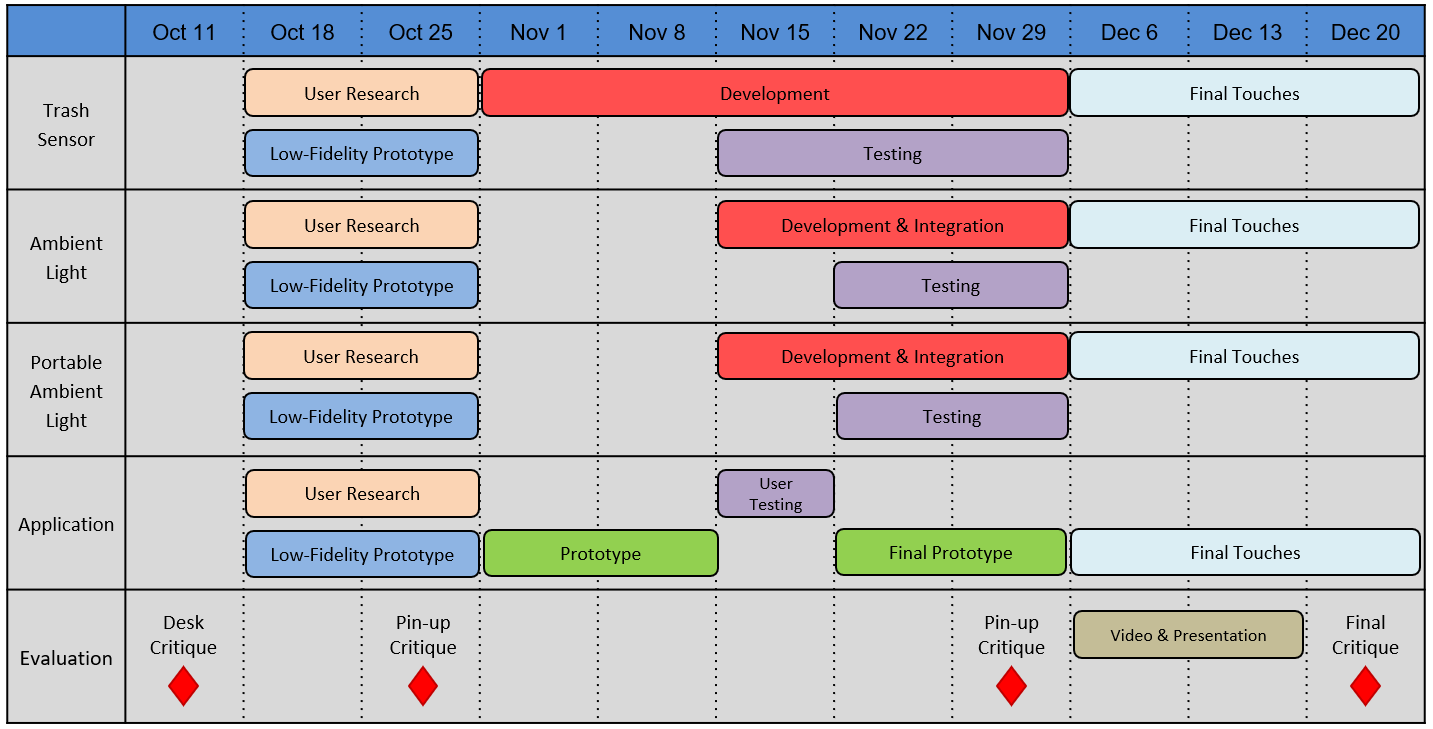
\includegraphics[width=.9\textwidth]{figures/schedule}
  \caption{Work schedule.}
\end{figure*}

\bibliographystyle{SIGCHI-Reference-Format}
\bibliography{mybib}

\end{document}

%%% Local Variables:
%%% mode: latex
%%% TeX-master: t
%%% End:
